\documentclass[a4paper,12pt]{article} 

% First, we usually want to set the margins of our document. For this we use the package geometry.
\usepackage[top = 2.5cm, bottom = 2.5cm, left = 2.5cm, right = 2.5cm]{geometry} 
\usepackage[T1]{fontenc}
\usepackage[utf8]{inputenc}

% The following two packages - multirow and booktabs - are needed to create nice looking tables.
\usepackage{multirow} % Multirow is for tables with multiple rows within one cell.
\usepackage{booktabs} % For even nicer tables.

% As we usually want to include some plots (.pdf files) we need a package for that.
\usepackage{graphicx} 

% The default setting of LaTeX is to indent new paragraphs. This is useful for articles. But not really nice for homework problem sets. The following command sets the indent to 0.
% \usepackage{setspace}
% \setlength{\parindent}{0in}
\usepackage{indentfirst}

% Package to place figures where you want them.
\usepackage{float}

% The fancyhdr package let's us create nice headers.
\usepackage{fancyhdr}

\usepackage{xcolor,amsmath,amsthm,algorithm2e,tikz,subcaption}
\RestyleAlgo{ruled}

\definecolor{myRed}{RGB}{211, 31, 17}
\definecolor{myOrange}{RGB}{244, 122, 0}
\definecolor{myLightTeal}{RGB}{98, 200, 211}
\definecolor{myDarkTeal}{RGB}{0, 113, 145}


% To make our document nice we want a header and number the pages in the footer.

\pagestyle{fancy} % With this command we can customize the header style.

\fancyhf{} % This makes sure we do not have other information in our header or footer.

\lhead{\footnotesize Algorithm Design and Analysis(H): Assignment 4}% \lhead puts text in the top left corner. \footnotesize sets our font to a smaller size.

%\rhead works just like \lhead (you can also use \chead)
\rhead{\footnotesize Mengxuan Wu} %<---- Fill in your lastnames.

% Similar commands work for the footer (\lfoot, \cfoot and \rfoot).
% We want to put our page number in the center.
\cfoot{\footnotesize \thepage} 

\begin{document}

\thispagestyle{empty} % This command disables the header on the first page. 

\begin{tabular}{p{15.5cm}}
{\large \bf Algorithm Design and Analysis(H)} \\
Southern University of Science and Technology \\ Mengxuan Wu \\ 12212006 \\
\hline
\\
\end{tabular}

\begin{center}
	{\Large \bf Assignment 4 \\ SPFA with Tarjan's quick disassembly trick}
	\vspace{2mm}

	{\bf Mengxuan Wu}
		
\end{center}  

\section*{Psuedocode}

\begin{algorithm}[H]
	\caption{SPFA with Tarjan's quick disassembly trick}
	\KwIn{Graph $G = (V, E)$, $s$, $t$}
	\KwOut{Shortest path from $s$ to all other vertices and whether there is a negative cycle}
	\BlankLine
	\SetKwFunction{FMain}{SPFA}
	\SetKwProg{Fn}{Function}{:}{}
	\Fn{\FMain{$G, s, t$}}{
		\ForEach{$v \in V$}{
			$dist[v] \leftarrow \infty$ \\
			$successor[v] \leftarrow \text{null}$ \\
		}
		$dist[t] \leftarrow 0$ \\
		\For{$i = 1$ \KwTo $|V| - 1$}{
			preprocess the preorder traversal of the Shortest Path Tree \\
			\ForEach{$v \in V$}{
				$dormant[v] \leftarrow false$ \\
			}
			\ForEach{$w \in V$}{
				\If{$dist[w]$ is updated in previous iteration and $dormant[w] = false$}{
					\ForEach{$(v, w) \in E$}{
						\If{$dist[v] > dist[w] + C_{vw}$}{
							$dist[v] \leftarrow dist[w] + C_{vw}$ \\
							$successor[v] \leftarrow w$ \\
							\If{$disassemble(v, w)$}{
								\Return{true} \\
							}
							$addChild(v, w)$ \\
						}
					}
				}
			}
			\If{no $dist[v]$ is updated in this iteration}{
				\Return{false} \\
			}
		}
		\Return{false} \\
	}
\end{algorithm}

\begin{algorithm}[H]
	\caption{Disassemble}
	\KwIn{Subtree root $v$, Parent $w$}
	\KwOut{Whether there is a negative cycle}
	\KwData{A preprocessed preorder traversal of the Shortest Path Tree of current iteration}
	\BlankLine
	\SetKwFunction{FMain}{disassemble}
	\SetKwProg{Fn}{Function}{:}{}
	\Fn{\FMain{$v, w$}}{
		$prev \leftarrow v.prev$ \\
		$currentLevel \leftarrow v.level$ \\
		$dormant[v] \leftarrow true$ \\
		$curr \leftarrow v.next$ \\
		\While{$curr.level > currentLevel$}{
			\If{$curr = w$}{
				\Return{true} \\
			}
			$dormant[curr] \leftarrow true$ \\
			$curr \leftarrow curr.next$ \\
		}
		$curr.prev \leftarrow prev$ \\
		$prev.next \leftarrow curr$ \\
	}
\end{algorithm}

\section*{Core idea}

The edges we specified with $successor$ are the edges that are used to represent the Shortest Path Tree (Once the algorithm finishes, we can find the shortest path following these edges).
This tree's root will be $t$, and the edges are directed from the children to the parent.
With such a setting, if we update the distance of a vertex $v$ in the $i$-th iteration, then we know all of its children are going to be updated in the $i+1$-th iteration.
This means updating these children in the $i$-th iteration is unnecessary, and we can skip them.

It also gives a convenient way to detect negative cycles. 
When we update the distance of a vertex $v$, we are adding an edge $(v, w)$ to the Shortest Path Tree.
If $w$ is one of the children of $v$, then there exists a cycle in the Shortest Path Tree.
The figure below shows the two cases when adding an edge $(v, w)$ to the Shortest Path Tree and removing the previous edge $(v, t)$.
\begin{figure}[H]
	\begin{subfigure}[t]{.5\textwidth}
		\centering
		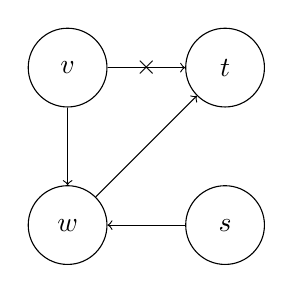
\begin{tikzpicture}
			\draw (0, 0) node [circle, draw, minimum size=1cm] (v) {$v$}; 
			\draw (0, -2) node [circle, draw, minimum size=1cm] (w) {$w$};
			\draw (2, 0) node [circle, draw, minimum size=1cm] (t) {$t$};
			\draw (2, -2) node [circle, draw, minimum size=1cm] (s) {$s$};
			\path [->] (v) edge (w);
			\path [->] (s) edge (w);
			\path [->] (w) edge (t);
			\path [->] (v) edge node {$\times$} (t);
		\end{tikzpicture}
		\caption{Will not cause negative cycle ($w$ is not a child of $v$)}
	\end{subfigure}
	\begin{subfigure}[t]{.5\textwidth}
		\centering
		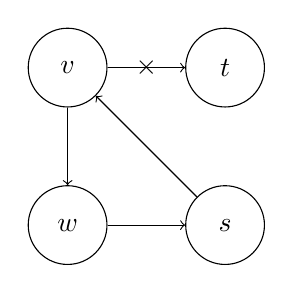
\begin{tikzpicture}
			\draw (0, 0) node [circle, draw, minimum size=1cm] (v) {$v$}; 
			\draw (0, -2) node [circle, draw, minimum size=1cm] (w) {$w$};
			\draw (2, 0) node [circle, draw, minimum size=1cm] (t) {$t$};
			\draw (2, -2) node [circle, draw, minimum size=1cm] (s) {$s$};
			\path [->] (v) edge (w);
			\path [->] (s) edge (v);
			\path [->] (w) edge (s);
			\path [->] (v) edge node {$\times$} (t);
		\end{tikzpicture}
		\caption{Will cause negative cycle ($w$ is a child of $v$)}
	\end{subfigure}
\end{figure}

Since there is a cycle, there will be an infinite loop with our algorithm and thus there must be a negative cycle.
Taking the same example, since $v$ is updated in the $i$-th iteration, then $v$ will be checked in the $i+1$-th iteration and $s$ will be updated.
This will cause $w$ to be updated in the $i+2$-th iteration, and $v$ will be updated again in the $i+3$-th iteration.
This will be an infinite loop.

Combining these two ideas, each time we update the distance of a vertex $v$, we can scan all its children.
If we find $w$, then we know there is a negative cycle.
If we don't, we mark all of them as dormant, and skip them in the current iteration.

\section*{Critical Process}

The critical process of the algorithm is the disassemble function.
I will use an example from reference \cite{article} to illustrate the process.

\begin{figure}[H]
	\begin{subfigure}{.5\textwidth}
		\centering
		\begin{tikzpicture}
			\draw (0, 0) node [circle, draw, minimum size=1cm] (v1) {};
			\draw (-3, -2) node [circle, draw, minimum size=1cm] (v2) {};
			\draw (0, -2) node [circle, draw, minimum size=1cm] (v3) {};
			\draw (3, -2) node [circle, draw, minimum size=1cm] (v4) {};
			\draw (-1.5, -4) node [circle, draw, minimum size=1cm] (v5) {};
			\draw (1.5, -4) node [circle, draw, minimum size=1cm] (v6) {};
			\path (v1) edge (v2);
			\path (v1) edge (v3);
			\path (v1) edge (v4);
			\path (v3) edge (v5);
			\path (v3) edge (v6);
		\end{tikzpicture}
		\caption{Shortest Path Tree}
	\end{subfigure}
	\begin{subfigure}{.5\textwidth}
		\centering
		\begin{tikzpicture}
			\draw (1,2) node [circle, draw, minimum size=1cm] (v0) {0};
			\draw (0, 0) node [circle, draw, minimum size=1cm] (v1) {1};
			\draw (-3, -2) node [circle, draw, minimum size=1cm] (v2) {2};
			\draw (0, -2) node [circle, draw, minimum size=1cm] (v3) {2};
			\draw (3, -2) node [circle, draw, minimum size=1cm] (v4) {2};
			\draw (-1.5, -4) node [circle, draw, minimum size=1cm] (v5) {3};
			\draw (1.5, -4) node [circle, draw, minimum size=1cm] (v6) {3};
			\path (v0) edge (v1)
			(v1) edge (v2)
			(v2) edge (v3)
			(v3) edge (v5)
			(v5) edge (v6)
			(v6) edge (v4)
			(v4) edge (v0);	
		\end{tikzpicture}
		\caption{Preorder traversal}
	\end{subfigure}
\end{figure}

We use an extra dummy vertex $v_0$ to avoid the special case when all the vertices are dormant.
The preorder traversal of the Shortest Path Tree help we define the subtrees by the level of the vertices.
For each vertex $v$, all the vertices in the subtree rooted at $v$ will have a level greater than $v$.
Also, this traversal will help us find the children of a vertex.
Since all the vertices are in a linked list, we can find the children of a vertex by scanning the linked list.

\section*{Complexity Analysis}

\subsection*{Time Complexity}

Since the disassemble function is traversing the Shortest Path Tree, in the worst case it will traverse all the vertices in the tree.
Since each node at most be marked as dormant once in a single iteration, the disassemble function will take $O(n + m)$ time.
The rest of the algorithm is the same as the normal SPFA algorithm.
Hence, the time complexity of each iteration is $O(m)$.
The SPFA algorithm will run for $n - 1$ iterations.
Overall, the time complexity is $O(mn)$.

\subsection*{Space Complexity}

The space will be required to store the distance, successor, and dormant status of each vertex.
Also, we need space to store the graph.
Hence, the graph storage will be the dominating factor, and the overall space complexity is $O(m + n)$.

\section*{Example}

\begin{center}
	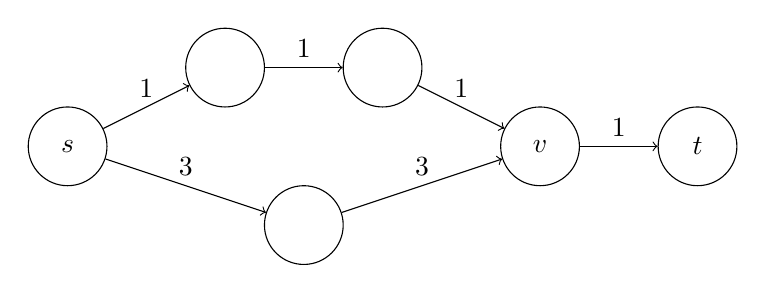
\begin{tikzpicture}
		\draw (0, 0) node [circle, draw, minimum size=1cm] (s) {$s$};
		\draw (2, 1) node [circle, draw, minimum size=1cm] (v1) {};
		\draw (4, 1) node [circle, draw, minimum size=1cm] (v2) {};
		\draw (3, -1) node [circle, draw, minimum size=1cm] (v3) {};
		\draw (6, 0) node [circle, draw, minimum size=1cm] (v4) {$v$};
		\draw (8, 0) node [circle, draw, minimum size=1cm] (t) {$t$};
		\path [->] (s) edge node [above] {1} (v1);
		\path [->] (v1) edge node [above] {1} (v2);
		\path [->] (s) edge node [above] {3} (v3);
		\path [->] (v2) edge node [above] {1} (v4);
		\path [->] (v3) edge node [above] {3} (v4);
		\path [->] (v4) edge node [above] {1} (t);
	\end{tikzpicture}
\end{center}

In this example, the shortest path from $s$ to $t$ is the upper path with length 4.
However, when we run the normal SPFA algorithm, we will get the lower path with length 7 first, then be corrected to the upper path in the next iteration.
This is because the lower path is shorter than the upper path.

With the SPFA algorithm with Tarjan's quick disassembly trick, we will mark the node $s$ as dormant when we find the lower path.
Hence, the distance of $s$ will not be updated in current iteration.
This will skip one update operation.
And in the next iteration, we will find the upper path and make the correct update in the next next iteration.

As this example shows, the SPFA algorithm with Tarjan's quick disassembly trick can avoid unnecessary updates and thus reduce the number of iterations, even when the graph contains no negative cycles.

\bibliographystyle{ieeetr}
\bibliography{reference}
\end{document}